\documentclass[serif,mathserif]{beamer}
\usepackage{amsmath, amsfonts, epsfig, xspace}
\usepackage{pstricks,pst-node}
\usepackage{multimedia}
\usepackage[normal,tight,center]{subfigure}
\setlength{\subfigcapskip}{-.5em}
\usepackage{beamerthemesplit}
\usetheme{lankton-keynote}
\usepackage{listings}

\author[Erik Lind\'en, erlinden@kth.se]{Erik Lind\'en}

\title[Automatic Differentiation in Ceres\hspace{2em}\insertframenumber/\inserttotalframenumber]{Automatic Differentiation in Ceres Solver}

\date{March 29, 2018} %leave out for today's date to be insterted

\institute{KTH / Tobii}

\begin{document}

\maketitle

\begin{frame}
  \frametitle{What is Ceres?}
  \begin{itemize}
  \item What is Ceres? \pause
  \item Ceres is an non-linear least squares optimizer. \pause
  \item Mostly for bundle adjustment. \pause
  \item What is bundle adjustment? \pause
  \item Given $N$ points observed by $C$ cameras, find the positions of the points and the poses of the cameras
  that minimized the mean squared back-projection error.
  \end{itemize}
\end{frame}

\begin{frame}
    \frametitle{Bundle adjustment example}
    \centering
    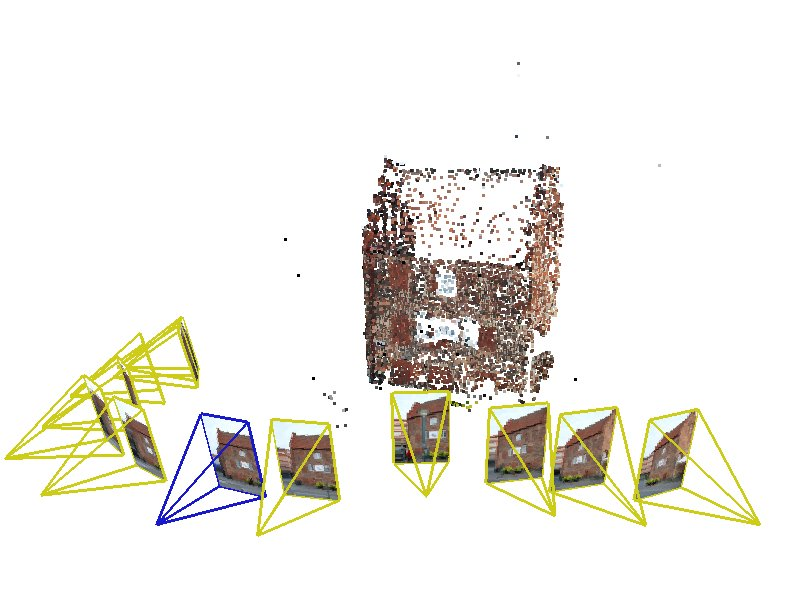
\includegraphics[width=1\textwidth]{Hus_rec.jpg}
\end{frame}

\begin{frame}
  \frametitle{Optimization problem}
  \begin{itemize}
  \item Minimize
  \[L(p, \theta) = \sum_{c=1}^C \sum_{i \in P_c} r(p_i, \theta_c, o_{c,i})^2 \]
  where  we have camera $c$ and point $i$.
  $P_c$ is the points seen by the camera, $p_i$ is the position of the point, $\theta_c$ is the pose of the camera,
  $o_{c,i}$ is where the camera saw the point and $r(\cdot)$ is the back-projection error. \pause
  \item Minimized with respect to all point positions $p$ and camera poses $\theta$. \pause
  \item How do we do that? 
  \end{itemize}
\end{frame}

\begin{frame}
  \frametitle{Solvers}
  \begin{itemize}
  \item Some may know Matlab's \texttt{lsqnonlin} (or scipy equivalent). \pause
  \item \texttt{lsqnonlin} uses the Jacobian of the residuals w.r.t. the parameters.
  For least-squares problems, this gives us the Hessian of the cost function for free
  \[
  L = \frac{1}{2} r^T r, \quad
  \frac{\delta L}{\delta x} = J^T r, \quad
  \frac{\delta^2 L}{\delta x^2} = J^T J
  \] \pause
  \item A second-order approximation of $L$ is
  \[  L(x + \triangle x) \approx L + J^T r \triangle x  + \frac{1}{2!}\triangle x^T J^T J \triangle x  \] \pause
  \item Taking the derivative w.r.t $\triangle x$ and setting it to zero gives
  \[ J^T J \triangle x = - J^T r \]
  \end{itemize}
\end{frame}

\begin{frame}
  \frametitle{Jacobians}
  \begin{itemize}
  \item How do we find the Jacobian $J$? \texttt{lsqnonlin} gives you two options: numeric or symbolic differentiation. \pause
  \item Numeric differentiation is slow and commits both cardinal sins of numerical analysis:
  \emph{``thou shalt not add small numbers to big numbers''}, and 
  \emph{``thou shalt not subtract numbers which are approximately equal''}. \pause
  \item Symbolic differentiation is tedious and error-prone. \pause
  \item But there is a third way...
  \end{itemize}
\end{frame}

\begin{frame}
  \frametitle{The chain rule}
  \begin{itemize} 
  \item Consider
  \[  y = f(g(h(x))) = f(g(w_1)) = f(w_2)  \] \pause
  \item The chain rule says
  \[  \frac{dy}{dx} = \frac{dy}{dw_2}\frac{dw_2}{dw_1}\frac{dw_1}{dx}  \] \pause
  \item In forward-mode automatic differentiation, we evaluate the chain rule from the inside out.
  \end{itemize}
\end{frame}

\begin{frame}
  \frametitle{Dual numbers}
  \begin{itemize} 
  \item Forward-mode automatic differentiation can be efficiently implemented using dual numbers.
  We replace the real number $x$ with $x + v \epsilon$, where $\epsilon$ is \emph{infinitesimal} such that $\epsilon^2=0$. \pause
  \item Then we can evaluate simple expressions like this
  \begin{align*}
  f(x) &= x^2 \\
  &= (x + v \epsilon)^2 \\
  &= x^2 + 2 x v \epsilon + \epsilon^2 \\
  &= x^2 + 2 x v \epsilon
  \end{align*} \pause
  \item In this case, the gradient is $2xv$.
  \end{itemize}
\end{frame}

\begin{frame}
  \frametitle{Dual numbers continued...}
  \begin{itemize} 
  \item We (usually) evaluate the expressions immediately, to get a numerical value.
  For example, let $x = 10$. Then we replace $x$ with $10 + 1\epsilon$. We have $v = 1$ since
  the gradient of $x$ with respect to $x$ is $1$. And then evaluate $đ$
  \begin{align*}
  f(10 + 1\epsilon) &= 10^2 + 2\cdot 10\cdot 1 \epsilon \\
  &= 100 + 20 \epsilon
  \end{align*} \pause
  \item So the value of $f(10)$ is $100$ and the gradient is $20$.
  \end{itemize}
\end{frame}

\begin{frame}
  \frametitle{Dual numbers continued...}
  \begin{itemize} 
  \item If we have more then one number, we introduce more infinitesimals
  \begin{align*}
  x &= x + v_1 \epsilon + v_2 \delta \\
  y &= y + u_1 \epsilon + u_2 \delta
  \end{align*} \pause
  \item By initializing, seeding, $v_1=1$, $v_2=0$ for $x$ and $u_1=0$, $u_2=1$ for $y$,
  we can compute gradients for both variables at the same time. \pause
  \item In general, each dual number needs to hold a vector of $N$ gradients, where $N$ is the number of parameters. \pause
  \item Though bundle adjustment is a special case...
  \end{itemize}
\end{frame}

\begin{frame}
  \frametitle{Sparsity in bundle adjustment}
  \begin{itemize}
  \item In bundle adjustment, the Jacobian gets a very special sparsity pattern,
  since any residual only depends on one point and one camera. \pause
  \item The dual numbers only need to track $3 + 3 +3 = 9$ gradients when computing a residual. \pause
  \item Ceres does a lot of algorithmic magic to leverage this special sparsity structure.
  \end{itemize}
\end{frame}

\begin{frame}[fragile]
  \frametitle{Implementation?}
  \begin{itemize}
  \item How does Ceres implement dual numbers? \pause
  \item 
    \lstset{language=C++}
\begin{lstlisting}
template<int N>
class Jet{
  ...
  double a;
  Eigen::Vector<double, N> v;
};
\end{lstlisting} \pause
  \item Almost all math operations are overloaded for \texttt{Jet}. \pause
  \item Your cost function must be templated on the value type.
  \end{itemize}
\end{frame}

\begin{frame}
  \frametitle{Forward vs. reverse mode AD}
  \begin{itemize}
  \item Forward mode automatic differentiation walks the chain rule inside out. \pause
  \item Most efficient for functions $f : \mathbb{R}^n \rightarrow \mathbb{R}^m$ where $m \gg n$. \pause
  \item Reverse mode automatic differentiation walks the chain rule from the outside in. \pause
  \item Most efficient for functions $f : \mathbb{R}^n \rightarrow \mathbb{R}^m$ where $m \ll n$. \pause
  \item When training neural networks, reverse mode automatic differentiation is called ``backprop''.
  \end{itemize}
\end{frame}

\begin{frame}
  \frametitle{Summary}
  \begin{itemize}
  \item There is a method to quickly and easily compute accurate gradients. \pause
  \item It is implemented in most languages.
  \end{itemize}
\end{frame}

\begin{frame}
  \frametitle{Further reading}
  \begin{itemize}
  \item The Wikipedia page. \pause
  \item Ceres' documentation. \pause
  \item \emph{Automatic Differentiation in Machine Learning: a Survey}.
  \end{itemize}
\end{frame}

\begin{frame}
  \frametitle{Questions?}
\end{frame}
\end{document}
